\section{Specification Languages}

\subsection{Property-based specification with QuickChick}
My first formal specification of \http was written as
QuickChick~\cite{quickchick} properties, which takes a trace of requests, and
determines whether the traces is valid per protocol specification, like that
shown in \autoref{fig:etag-tester}.  The specification implemented a constraint
solving logic by hand, making it hard to scale when the protocol becomes more
complex, as discussed in \autoref{sec:challenges}

\subsection{Model-based specification with ITrees}
To write specifications for protocols' rich semantics, I employed ``interaction
tree'' (ITree), a generic data structure for representing interactive programs,
introduced by \textcite{itree}.  ITree enables specifying protocols as monadic
programs that model valid implementations' possible behavior.  The model program
can be interpreted into a tester program, to be discussed in
\autoref{sec:spec-to-test}.

\begin{figure}
  \begin{lstlisting}[style=customcoq]
CoInductive itree (E : Type -> Type) (R : Type) :=
| Ret (r : R)
| Vis {X : Type} (e : E X) (k : X -> itree E R)
| Tau (t : itree E R).

Inductive event (E : Type -> Type) : Type :=
| Event : forall X, E X -> X -> event E.

Definition trace E := list (event E)

Inductive is_trace E R
  : itree E R -> trace E -> Prop := ...
  (* straightforward definition omitted *)
 \end{lstlisting}
  \caption{Interaction trees and their traces of events.}
  \label{fig:itrees}
\end{figure}

Figure~\ref{fig:itrees} defines the type \ilc{itree E R}.  The definition is
\textit{coinductive}, so that it can represent potentially infinite sequences of
interactions, as well as divergent behaviors.  The parameter \ilc{E} is a type
of \textit{external interactions}---it defines the interface by which a
computation interacts with its environment.  \ilc{R} is the \textit{result} of
the computation: if the computation halts, it returns a value of type \ilc{R}.

There are three ways to construct an ITree. The \ilc{Ret r} constructor
corresponds to the trivial computation that halts and yields the value
\ilc{r}. The \ilc{Tau t} constructor corresponds to a silent step of
computation, which does something internal that does not produce any visible
effect and then continues as \ilc{t}.  Representing silent steps explicitly with
\ilc{Tau} allows us, for example, to represent diverging computation without
violating Coq's guardedness condition~\cite{coinduction}:

\begin{lstlisting}[style=customcoq]
CoFixpoint spin {E R} : itree E R := Tau spin.
\end{lstlisting}

The final, and most interesting, way to build an ITree is with the \ilc{Vis X e
  k} constructor.  Here, \ilc{e : E X} is a ``visible'' external effect
(including any outputs provided by the computation to its environment) and
\ilc{X} is the type of data that the environment provides in response to the
event.  The constructor also specifies a continuation, \ilc{k}, which produces
the rest of the computation given the response from the environment.  \ilc{Vis}
creates branches in the interaction tree because \ilc{k} can behave differently
for distinct values of type \ilc{X}.

Here is a small example that defines a type \ilc{IO} of output or input
interactions, each of which works with natural numbers.  It is then
straightforward to define an ITree computation that loops forever, echoing each
input received to the output:

\begin{lstlisting}[style=customcoq]
Variant IO : Type -> Type :=
| Input  : IO nat
| Output : nat -> IO ().

CoInductive echo : itree IO () :=
  Vis Input (fun x => Vis (Output x) (fun _ => echo)).
\end{lstlisting}

\section{From Specification to Tester}
\label{sec:spec-to-test}
From an ITree specification, I conducted ``offline'' testing, which takes a
trace and determines its validity~\cite{cpp19}, and ``online'' testing, where
the specification is derived into a client program that validates the system
under test interactively~\cite{issta21}.

\subsection{Offline testing of swap server}
I started with testing a simple ``swap server''~\cite{cpp19}, specified in
\autoref{fig:linear-spec}.  The specification says that the server can either
accept a connection with a new client (\ilc{obs_connect}) or else receive a
message from a client over some established connection (\ilc{obs_msg_to_server}
\ilc{c}), send back the current stored message (\ilc{obs_msg_from_server}
\ilc{c} \ilc{last_msg}), and then start over with the last received message as
the current state.

\begin{figure}
\begin{lstlisting}[style=customcoq]
CoFixpoint linear_spec' (conns : list connection_id)
           (last_msg : bytes) : itree specE unit :=
  or ( (* Accept a new connection. *)
       c <- obs_connect;;
       linear_spec' (c :: conns) last_msg )
     ( (* Exchange a pair of messages on a connection. *)
       c <- choose conns;;
       msg <- obs_msg_to_server c;;
       obs_msg_from_server c last_msg;;
       linear_spec' conns msg ).

Definition linear_spec := linear_spec' [] zeros.
\end{lstlisting}
\caption{Linear specification of the swap server.  In the \ilc{linear_spec'}
  loop, the parameter \ilc{conns} maintains the list of open connections, while
  \ilc{last_msg} holds the message received from the last client (which will be
  sent back to the next client).  The server repeatedly chooses between
  accepting a new connection or doing a receive and then a send on some existing
  connection picked in the list \ilc{conns}.  The linear specification is
  initialized with an empty set of connections and a message filled with zeros.}
\label{fig:linear-spec}
\end{figure}

To test this swap server, I wrote a client program that interacts with the
server and produces a trace of requests and responses, and a function that
determines whether the trace $t$ is a trace of the linear specification $s$ {\it
  i.e.} whether \ilc{is_trace s t} in \autoref{fig:itrees} holds.

To network nondeterminism, the checker enumerates all possible server-side
message orders that can explain the client-side observations, and checks if any
of them satisifes the protocol specification.

\subsection{Online testing of HTTP}
To test protocols with internal nondeterminism ({\it e.g.} HTTP) effectively, I
introduced a symbolic representation for the server's invisible choices, as
shown in \autoref{fig:if-match-model}.  I then defined a TCP network model in
\autoref{fig:tcp-model}.  Combining the server and network models produces a
model program that exhibits all valid observations, considering both internal
and network nondeterminism.

\begin{figure}
\begin{lstlisting}[style=customcoq]
(* matches : (etag * exp etag) -> exp bool *)
(* IF      : (exp bool * T * T) -> T       *)
let put (k    : key,
         t    : etag,
         v    : value,
         data : key -> value,
         xtag : key -> exp etag) =
    IF (matches(t, xtag[k]),
    (* then *)
       xt := fresh_tag();
       let xtag' = update(xtag, k, xt) in
       let data' = update(data, k, v)  in
       return (OK, xtag', data'),
    (* else *)
       return (PreconditionFailed, xtag, data))
\end{lstlisting}
\caption{Symbolic model handling conditional PUT request.  The model maintains
  two states: \ilc{data} that maps keys to their values, and \ilc{xtag} that
  maps keys to symbolic variables that represent their corresponding ETags.
  Upon receiving a PUT request conditioned over ``If-Match: \ilc{t}'', the
  server should decide whether the request ETag \ilc{matches} that stored in the
  server.  Upon matching, the server processes the PUT request, and represents
  the updated value's ETag as a fresh variable.
}
\label{fig:if-match-model}
\end{figure}

\begin{figure}
\begin{lstlisting}[style=customcoq]
let tcp (buffer : list packet) =
    let absorb =
        pkt := recv();
        tcp (buffer ++ [pkt]) in
    let emit =
        let pkts = oldest_in_each_conn(buffer) in
        pkt := pick_one(pkts);
        send(pkt);
        tcp (remove(pkt, buffer)) in
    or (absorb, emit)
\end{lstlisting}
\caption{Network model for concurrent TCP connections.  The model maintains a
  \ilc{buffer} of all packets en route.  In each cycle, the model may
  nondeterministically branch to either absorb \ilc{or} emit a packet.  Any
  absorbed packet is appended to the end of buffer.  When emitting a packet, the
  model may choose a connection and send the oldest packet in it.  }
\label{fig:tcp-model}
\end{figure}

From the server and network models, I derived a tester client that interacts
with servers over the network, and validates the observations against the
protocol specification, as shown in \autoref{fig:framework}.

Using this automatially derived tester program, I have found violations against
HTTP/1.1 in the latest version of both Apache and Nginx.  More details are
explained in \textcite{issta21}.

\subsection{Key innovation}
To solve the problem of ``determinining whether an observation is explainable by
a nondeterministic program'', I reduced it into a constraint
satisfiability: Although the tester doesn't know the server and network's exact
choices, it can gain some knowledge of these invisible choices by observing the
trace of messages.  If the invisible choices are represented as symbolic
variables, then an observed trace is valid if there exists some value for the
variables that explains this trace, which can be determined by a constraint
solver.

\begin{figure}
  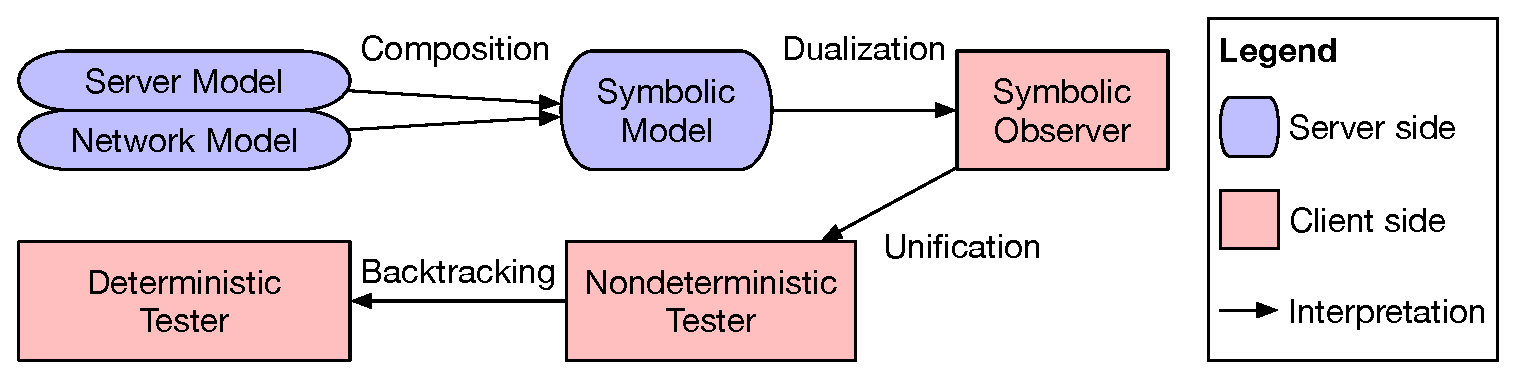
\includegraphics[width=\linewidth]{figures/framework}
  \caption{Deriving tester program from specification}
  \label{fig:framework}
\end{figure}
